\section{Modeling}
\label{sec:modeling}

To test whether it is possible to prioritize PRs we have designed a service that automatically tries to do just that.

\subsection{Features}
\label{sec:features}

For creating system that automatically creates an ordered list of PRs, we tried to use a machine algorithm that ranks the incoming PRs according a set of features.
Most of the features we use are based on features that are used by many integrators to manually sort their PRs \cite{GZSD15}.

\begin{description}
\item[Age]
The number of minutes between the moment the PR was opened to the current time.
There is a large group of integrators that take a PR's age into account when manually prioritizing their PRs.

\item[Target Branch]
The name of the branch the PR is targeting in the base repository.
It makes sense to use the target branch not as string, but as a categorical variable.
Unfortunately the ML algorithm chokes if there is a new branch value that was not part of the training data.
Therefore this feature is not included in the training data at all, but it is still available for manual sorting (see visualizer in section~\ref{sec:architecture}).

\item[Core Member]
A boolean value indicating whether the author of the pull request is a core member of the project.
Some integrators value PRs of members more than those of non-members.

\item[Intra-Branch]
A boolean value indicating whether the pull request is coming from another branch of the same base project.
Creating these kind of PRs requires write access to the repository, so they can only be created by core members.

\item[Contains Fix]
A boolean value indicating whether the pull request contains some sort of bug fix rather than e.g. a feature.
This is really just an indication as the value is only true if the PR contains the string ``fix'' in its title.
In general PRs with a fix are prioritized over other PRs.

\item[Contribution Rate]
The number of commits that is already included in the project \emph{and} authored by the pull requester divided by the total number of commits in the project.
I.e. the contribution rate of the PR author.
There are integrators that look at PRs of known contributers first, their code is of known quality and often faster to review.
On the other hand there are also integrators that value PRs of new contributors more than those of known contributers.
The rationale behind this is that new contributers are feeling more valued when they receive a fast response on their PR.
Possibly will that feeling encourage them to continue to contribute the to project.

\item[Accept rate]
The number of accepted (i.e. merged) pull requests authored by the current pull requester divided by the total number of PRs he/she authored.
I.e. the accept rate of the PR author.
A high accept rate can indicate that the author already gained some trust by the integrator, which can result in a higher prioritity.
This feature suffers possibly from accuracy problems, as it is difficult to determine whether a PR is actually merged or not.
A pull request can be merged in different ways \cite{GPD14}.
A merge performed via the GitHub interface is easy to detect, but a PR which is squashed to one commit before the merge is difficult to detect.

\item[Comments]
There are different types of comments that can be made regarding a pull request.
This feature counts the number of comments on the issue that is automatically created along the pull request.
Usually a general dicussion about the PR takes place within the issue.
The number of comments might indicate whether a PR needs more/less attention.

\item[Review Comments]
Review comments are comments on a portion of the unified diff of a pull request.
These are separate from issue comments, which do not reference a portion of the unified diff.
This feature counts the number of review comments on a PR.

\item[Last Comment Mention]
A boolean value indicating whether the last comment on a request (regardless of the comment type) contains a mention to a GitHub user.
A comment with a mention contains ``@username'' anywhere in the body of the comment.
The mention suggests that the user who is mentioned needs to take action.

\item[Additions]
The number of lines added by the pull request.
Together with the following three features it captures the size of a PR.
A very large group uses the size of the change to manually prioritize their PRs.

\item[Deletions]
The number of lines deleted by the pull request.

\item[Commits]
The number of commits contained by the pull request.

\item[Files]
The number of files changed by the pull request.

\item[Has Test Code]
A boolean value indicating whether the pull request contains changes to test files.
Some projects have a extensive test suite.
In these projects it is often expected that new PRs contain tests for the code they add.
The heuristic used for the test code detection is simple, the value of the feature is true if the PR changes at least one file with ``test'' or ``spec'' in its file name.

\item[Pairwise conflicts]
When the conflicts among other pending PRs are known, it can be used to determine a merge order in which the number of conflicts is reduced.
The actual number of conflicts is not reduced, but they can be concentrated in a particular merge action.
Figure~\ref{fig:conflicts-1} and \ref{fig:conflicts-3} show an example of the same set of three PRs but with different merge orders which result in a different amount of merge conflicts.
Pairwise conflicts are only checked among PRs which target the same branch, but nevertheless the amount of pairs can be very high.
In the worst case, i.e. when all PRs target the same branch, the number of pairs to be checked is $O(n^2)$.

A possible value of this feature could be the number of conflicts between other pending PRs.
However, since checking the pairwise conflicts takes quadratic time it would take a large amount of time to create the training data which requires multiple time windows for each pull request.
It boils down to $O(n^2 \cdot m)$ where $m$ is the average number of time windows per PR.
Because of this time complexity, we decided to leave this feature out of the ML algorithm and only make it available for manual sorting.

\begin{figure}
  \centering
  % Trim option's parameter order: left bottom right top
  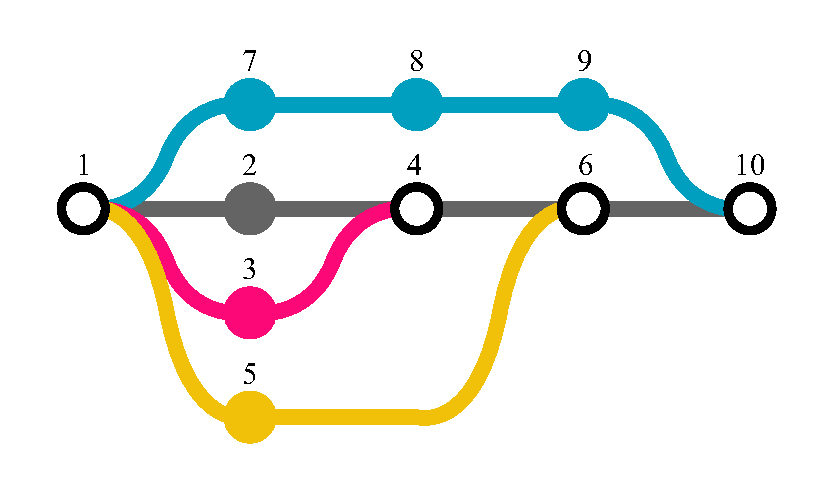
\includegraphics[height=25mm, clip ,trim = 0mm 7mm 0mm 7mm]{../figs/conflicts-1.pdf}
  \caption[Merge diagram with one conflict]
   {Merge diagram with one merge conflict.
   Consider the following conflicted commit pairs: $(2,7)$, $(3,8)$, $(5,9)$.
   The conflicts occur only in merge commit $10$.}
  \label{fig:conflicts-1}
\end{figure}

\begin{figure}
  \centering
  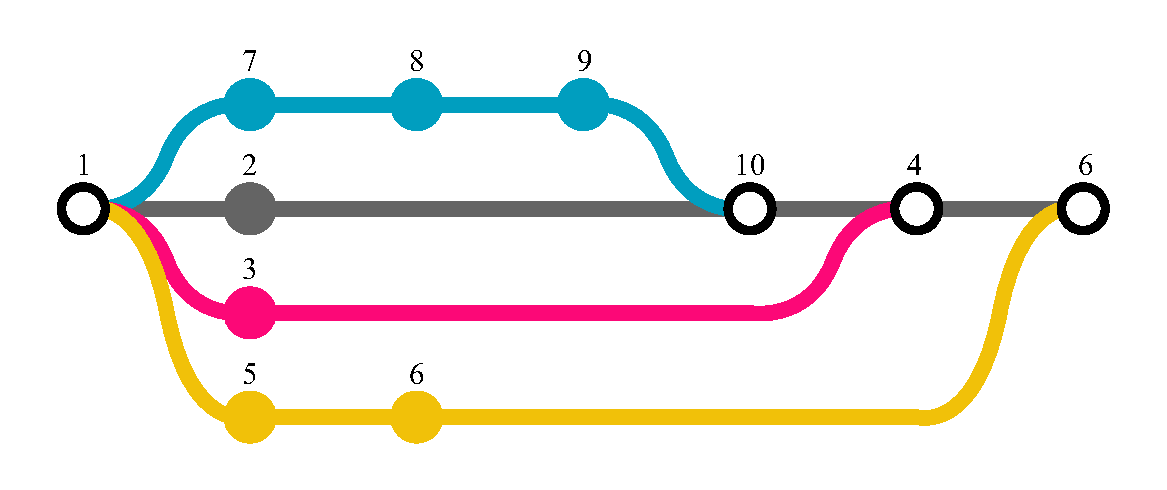
\includegraphics[height=25mm, clip ,trim = 0mm 7mm 0mm 7mm]{../figs/conflicts-3.pdf}
  \caption[Merge diagram with three merge conflicts]
   {Merge diagram with three merge conflicts.
   Consider the following conflicted commit pairs: $(2,7)$, $(3,8)$, $(5,9)$.
   The conflicts occur in each of the three merge commits $10,4,6$.}
  \label{fig:conflicts-3}
\end{figure}

\end{description}

\subsection{Training data}
\label{sec:training}

With the features described in the previous section we construct the training data.
For reasons discussed earlier we do not include the \emph{target branch} and \emph{pairwise conflicts} features.
There are different approaches of applying the pull-based development model \cite{GPD14}.
Because of this we create a different training set for every different GitHub project.

To train a prediction model so that it recognizes PRs that need attention, we have to provide it with actual examples of pull requests that we consider important.
We define important pull requests as follows: the current state of a pull request is important when an action follows on that PR.
An action can either be a merge, close, comment or review comment action.
To find out what the important states were, we have to dig into the past of previously closed PRs.
All the available information about the closed pull requests is extracted from \ghtorrent.
To determine the state of PRs in the past we take a systematic approach by dividing the lifetime of each PR into time windows.
The windows, with an interval of a day, contain a snapshot of the PR at the beginning of the window.
A PR's snapshot consists of its commits, comments and author info at the time.
Now that every PR is broken down into a list of consectutive snapshots, we can add information about the importance.
When an action is carried out within a certain time window, the snapshot contained in that window is marked as \emph{important}.
Snapshots of time windows that don't have any actions are not marked as important.
The final training data consists of these snapshots, where each snapshot is a row in the training data.
